In this section we present our rationale for selecting the systems we studied and present our data extraction and analysis approach.


In this paper, we aim to find the unstable logs in a system for easier management of log processing tools. We cloned locally over 15 projects which had more than 10,000 commits in their git repository. We also verify if the projects utilize a bug tracking system like 'JIRA' or `Bugzilla' because, this helps to tag commits to specific development activities (i.e., bug fix, improvement, new-features). We use the `grep' command to recursively search for all log lines within `.java' files in each project in the cloned repositories. We picked the top four projects with the highest log line count. The four open source projects are: Liferay, Camel, ActiveMQ and CloudStack. All studied systems have extensive system logs and Table~\ref{tba:overviewsystems} presents an overview of the systems.

\begin{table}[tbh]
\centering \protect\caption{An overview of all studied systems}


\label{tba:overviewsystems} %
\begin{tabular}{lllll}
\hline 
Projects  & Liferay  & Camel  & ActiveMQ  & CloudStack \tabularnewline
\hline 
Starting release  & 6.1.0-b3  & 1.6.0  & 4.1.1  & 2.1.3 \tabularnewline
End release  &7.0.0-m3  & 2.11.3  & 5.9.0  & 4.2.0 \tabularnewline
Total \# of releases   & 24  & 43  & 19 & 111 \tabularnewline
Total added code  & 3.9M  & 505k  & 261k  & 1.09M \tabularnewline
Total deleted code  & 2.8M  & 174k  & 114k  & 750K \tabularnewline
Total \# added logs  & 10.4k  & 5.1k  & 4.5k  & 24k \tabularnewline
Total \# deleted logs  & 8.1k  & 2.4k  & 2.3k  & 17k \tabularnewline
\hline 
\end{tabular}
\end{table}

\textbf{Liferay}\footnote[1]{http://www.liferay.com/}:  Liferay is a free and open source enterprise project written in Java. It provides platform features which are used in development of websites and portals.
% We select liferay as it is one of the leading platforms for platform development~\cite{LiferayGartner} and has growing user base~\cite{LiferayUser}.
  It also has an extensive issue tracking system in JIRA which helps in categorizing the commits as bug fixes, improvements, . We study the releases from 6.1.0 to 7.0.0-m3 which cover more than three years of development from 2010 to 2014

%Hadoop is an open source software framework for distributed storage and for the processing of big data on clusters. Hadoop uses the MapReduce data-processing paradigm. The logging characteristics of Hadoop have been studied in prior research~\cite{IanWCRE,EMSEIAN,IanContextinformation}. We study the releases from Hadoop 0.20.1 to 2.2.0.


\textbf{Camel}\footnote[2]{http://camel.apache.org/}: Camel is an open source integration platform based on enterprise integration patterns. We analyze Camel release 1.6 to 2.11.3 which cover more than five years of development from 2009 to 2013. 
\begin{figure*}
	\centering
	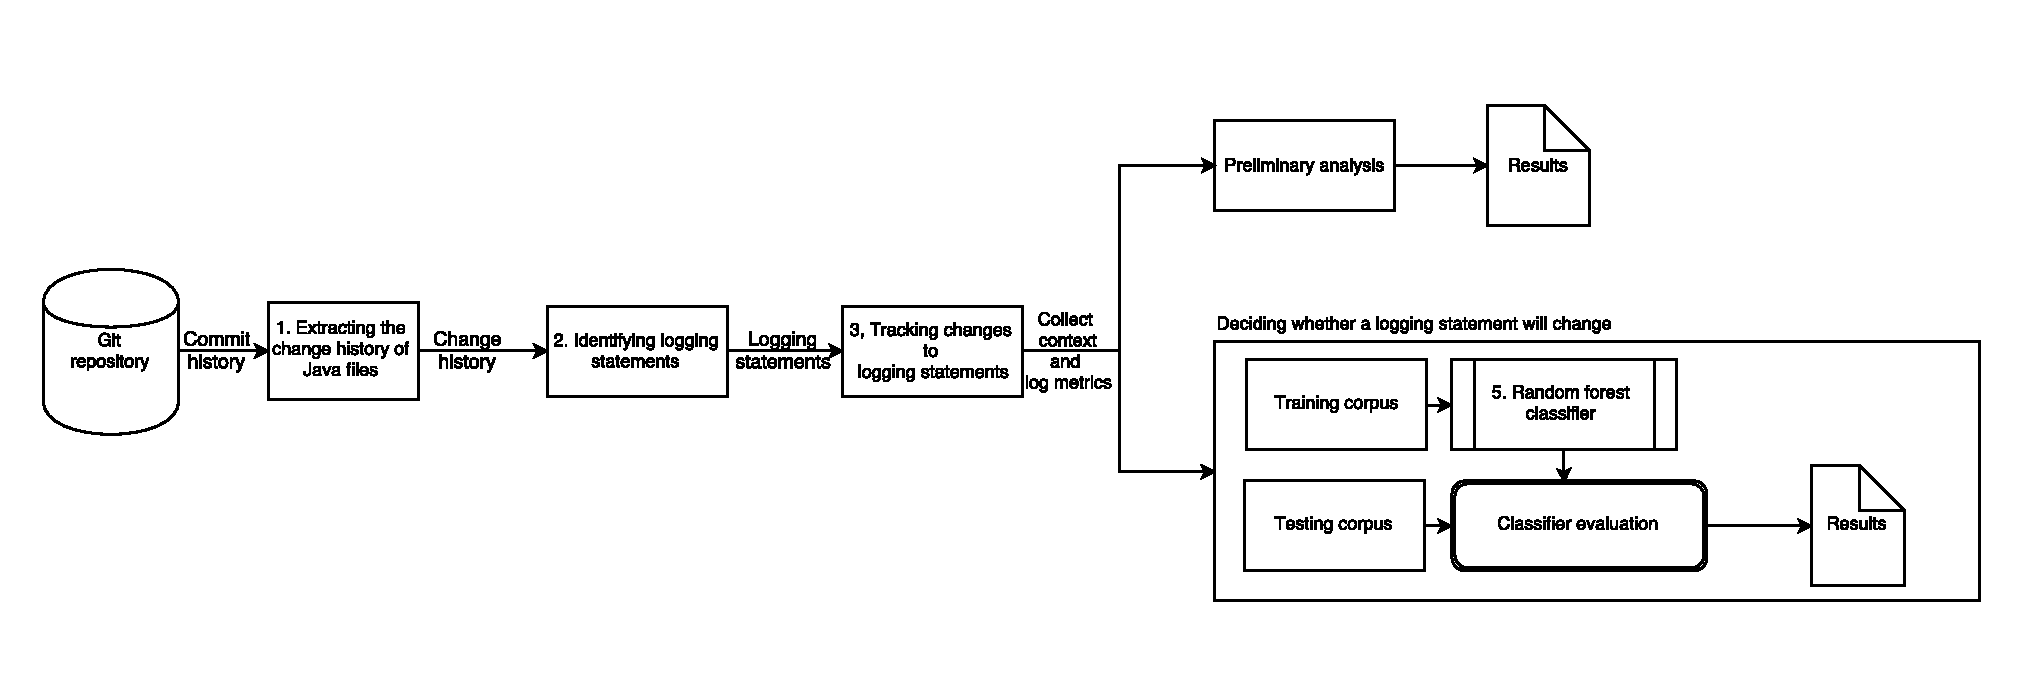
\includegraphics[width=1.7\columnwidth,height=0.50\columnwidth]{LogGenalogyMethdology}
	\caption{Overview of the data extraction and case study approach}
	\label{fig:LGmethod}
\end{figure*}



\textbf{ActiveMQ}\footnote[3]{http://activemq.apache.org/}: ActiveMQ is an open source message broker and integration patterns server. We covered ActiveMQ release 4.1.1 to 5.9.0 which cover more than 6 years of development from 2007 to 2013.


\textbf{CloudStack}\footnote[4]{https://cloudstack.apache.org/}: Apache CloudStack is open source software designed to deploy and manage large networks of virtual machines, as a highly available, highly scalable Infrastructure-as-a-Service (IaaS) cloud computing platform. We covered CloudStack release 2.1.3 to 4.20 which cover more than 3 year of development from 2010 to 2014.


Figure~\ref{fig:LGmethod} shows a general overview of our approach, which consists of four steps: (1) We mine the git repository of each studied system to extract all commits made for each file.(2) We identify the log changes in the extracted files. (3) We track the changes made to each log across the commits. (4) We extract the JIRA issues for the commits and collect the developer metrics when there is a log change in the commit.  We use a statistical tool R~\cite{ihaka1996r}, to perform experiments on the data to answer our research questions. 

\subsection{Study Approach}

 In the reminder of this section we describe the each of these steps.

\subsubsection{Extracting Code Evolution}
In order to find the stability of logs we have to identify all the `Java' files in our studied systems. To achieve this, we clone the \emph{master} branch of the git repository of each studied system locally. We use the `find' command to recursively find all the files which end with pattern `*.java'. To remove the \textsl{Java Test} files, we use `grep' command to filter all files which have `test' or `Test' in their pathname.

 After collecting all the Java files from the four studied systems, we use their git repository to obtain all the changes made to the file within the time-frame discussed above. We use the `follow' option to track the file even when they are renamed or relocated within our studied systems. We flatten all the changes made to files to include the changes made in different branches but exclude the final merging commit. Using this approach, we obtain a complete history of each \emph{Java} file. 

\subsubsection{Identifying Log Changes}
From the extracted code evolution data for each \emph{Java} file, we identify all the log changes made in the commits. To identify the log statements in the source code, we manually sample some commits from each studied system and identify the logging library used to generate the logs. We find that the studied systems use \textsl{Log4j}\footnote{http://logging.apache.org/log4j/2.x/}~\cite{EMSEIAN} and \textsl{Slf4j}\footnote{http://www.slf4j.org/} widely and \textsl{logback}\footnote{http://logback.qos.ch/} sparingly. Using this information we identify the common method invocations that invoke the logging library. For example in  ActiveMQ and Camel a logging library is invoked by method named `LOG' as shown below.
\hypobox{ LOG.debug(``Exception detail", exception);}

In CloudStack it is usually done through `\_logger' as follows.

\hypobox{\_logger.warn(``Timed out: " + buildCommandLine(command));}

As projects can have multiple logging libraries throughout its life-cycle, we use regular expressions to match all the common log invocation patterns (i.e., `LOG',`log',`\_logger',`LOGGER',`Log'). We count every such invocation of a logging library as a log.


\subsubsection{Tracking Log Changes}
After identifying all the log changes made to a file across multiple commits, we track each log individually to find out whether it has changed in subsequent revisions. We first collect all the logs present in a file at the first commit, which form the initial set of logs for the file. Every subsequent commit which has changes to a log appears as an added and deleted log in \textsl{git}. To track these log changes made, we used the Levenshtein ratio~\cite{levenshteinratio}.

To calculate Levenshtein ratio for a pair of added and deleted logs, we first remove the logging method (e.g., LOG) and compare the remaining text. We set a minimum threshold of 0.5 for a pair of added and deleted logs to be considered modified. We set 0.6 because there is atleast 60\% similarity between the pair. We find that when the threshold is set lower there are more false positives and when set higher we miss log modifications. When an added log has levenshtein ratio higher than 0.6 with multiple deleted logs, we consider the pair with highest levenshtein ratio. 

 For example in the logs shown below, we remove the logging method (i.e., LOG) and find that the Levenshtein ratio between the added and deleted pair is 0.86. Hence, this log change is categorized as a log modification.  
 \hypobox{+      LOG.debug(``Call: " +method.getName()+`` took "+ callTime + ``ms");\\ 
 	-        LOG.debug(``Call: " +method.getName()+ `` " + callTime);} 


If the added log does not match any log in our initial set, it is considered as a new log addition and is added to the initial set for tracking in future commits. From this we can track how many times a log is changed and how many commits are made between the changes. 


\subsubsection{Match JIRA to Log Changes}

Using the commit data, we also track the JIRA issues to extract the developer metrics such as developer experience, number of developers involved, issue priority. To achieve this, we extract the JIRA issue IDs from commit messages and use the JIRA repository to extract the JIRA issue. The JIRA issue contains information about the issue such as, type (i.e., bug, improvement, new-feature, task), priority, resolution time and developer information such as number of comments and number of developers involved in the JIRA discussion. We use this information along with code and log churn metrics for answering our research questions. 




 







